% !TEX program = xelatex
\documentclass[11pt,a4paper]{article}

\usepackage[a4paper,top=22mm,bottom=24mm,left=23mm,right=23mm,headheight=22pt]{geometry}
\usepackage{fontspec}
\usepackage[english]{babel}
\setmainfont{Georgia}
\setsansfont{Avenir Next}
\setmonofont{Andale Mono}[Scale=0.86]
\usepackage{microtype}
\usepackage{amsmath,amssymb}
\usepackage{booktabs,tabularx,longtable,array,multirow}
\usepackage{siunitx}
\sisetup{locale=US,group-separator={\,},group-minimum-digits=4,detect-all}
\usepackage{graphicx}
\usepackage{xcolor}
\usepackage{tikz}
\usetikzlibrary{arrows.meta,positioning,fit,calc,babel}
\usepackage{pgfplots}
\pgfplotsset{compat=1.18}
\usepackage[most]{tcolorbox}
\usepackage{enumitem}
\usepackage{caption}
\usepackage{fancyhdr}
\usepackage{titlesec}
\usepackage{hyperref}
\usepackage{xurl}
\usepackage[nameinlink,noabbrev]{cleveref}

\definecolor{navy}{HTML}{17324D}
\definecolor{blue}{HTML}{176B87}
\definecolor{teal}{HTML}{159A9C}
\definecolor{gold}{HTML}{E3A72F}
\definecolor{red}{HTML}{C64B4B}
\definecolor{ink}{HTML}{24313B}
\definecolor{muted}{HTML}{667784}
\definecolor{paper}{HTML}{F5F8FA}
\definecolor{line}{HTML}{D8E1E7}

\hypersetup{
  colorlinks=true,
  linkcolor=navy,
  citecolor=blue,
  urlcolor=blue,
  pdftitle={Hourly Electricity Demand Forecasting: Model Training and Experimental Results},
  pdfauthor={energy-demand-forecasting-foundation-models project}
}

\titleformat{\section}{\Large\bfseries\sffamily\color{navy}}{\thesection}{0.7em}{}
\titleformat{\subsection}{\large\bfseries\sffamily\color{blue}}{\thesubsection}{0.65em}{}
\titleformat{\subsubsection}{\normalsize\bfseries\sffamily\color{ink}}{\thesubsubsection}{0.6em}{}
\titlespacing*{\section}{0pt}{2.0ex plus .4ex}{1.0ex}
\titlespacing*{\subsection}{0pt}{1.6ex plus .3ex}{.7ex}

\pagestyle{fancy}
\fancyhf{}
\fancyhead[L]{\small\sffamily\color{muted} Electricity Demand Forecasting}
\fancyhead[R]{\small\sffamily\color{muted} Training and Results Report}
\fancyfoot[C]{\small\sffamily\color{muted}\thepage}
\renewcommand{\headrulewidth}{0.3pt}
\renewcommand{\headrule}{\hbox to\headwidth{\color{line}\leaders\hrule height \headrulewidth\hfill}}

\setlist[itemize]{leftmargin=1.4em,itemsep=.25em,topsep=.35em}
\setlist[enumerate]{leftmargin=1.5em,itemsep=.25em,topsep=.35em}
\renewcommand{\arraystretch}{1.15}
\setlength{\parindent}{0pt}
\setlength{\parskip}{0.55em}
\emergencystretch=2.5em

\newcommand{\code}[1]{\texttt{\detokenize{#1}}}
\newcommand{\best}[1]{\textbf{\color{navy}#1}}
\newcommand{\sourcepath}[1]{\texttt{\footnotesize\detokenize{#1}}}
\newcolumntype{Y}{>{\raggedright\arraybackslash}X}
\newcolumntype{R}{>{\raggedleft\arraybackslash}X}

\newtcolorbox{finding}[1][]{
  enhanced,breakable,colback=paper,colframe=teal,boxrule=.7pt,
  arc=2mm,left=3mm,right=3mm,top=2.2mm,bottom=2.2mm,
  fonttitle=\bfseries\sffamily,coltitle=navy,title={#1}}
\newtcolorbox{caution}[1][]{
  enhanced,breakable,colback=gold!7,colframe=gold!80!black,boxrule=.7pt,
  arc=2mm,left=3mm,right=3mm,top=2.2mm,bottom=2.2mm,
  fonttitle=\bfseries\sffamily,coltitle=ink,title={#1}}

\begin{document}
\pagenumbering{gobble}

% -----------------------------------------------------------------------------
% Cover
% -----------------------------------------------------------------------------
\begin{titlepage}
  \thispagestyle{empty}
  \begin{tikzpicture}[remember picture,overlay]
    \fill[navy] (current page.north west) rectangle ([yshift=-90mm]current page.north east);
    \fill[teal] ([yshift=-90mm]current page.north west) rectangle ([yshift=-93mm]current page.north east);
    \fill[paper] ([yshift=20mm]current page.south west) rectangle (current page.south east);
  \end{tikzpicture}

  \vspace*{12mm}
  {\sffamily\bfseries\color{white}\fontsize{27}{32}\selectfont
  Hourly Electricity\par
  Demand Forecasting\par}
  \vspace{3mm}
  {\sffamily\color{white}\fontsize{14}{18}\selectfont
  Training, Fine-tuning, and Comparative Evaluation\par
  of Time-series Foundation Models\par}

  \vspace{30mm}
  \begin{tcolorbox}[enhanced,colback=white,colframe=line,boxrule=.6pt,arc=2mm,
    left=6mm,right=6mm,top=5mm,bottom=5mm,shadow={1mm}{-1mm}{0mm}{black!8}]
    \begin{tabularx}{\textwidth}{@{}Y R@{}}
      \textbf{Dataset} & Monash \code{electricity_hourly}\\
      \textbf{Scope} & 321 series, 26,304 hours per series\\
      \textbf{Forecasting task} & 5 windows $\times$ 168 hours\\
      \textbf{Primary metric} & MASE ($m=24$)\\
      \textbf{Recommended model} & \code{chronos_bolt_base_ft}\\
      \textbf{Compute environment} & NVIDIA A100-SXM4-40GB\\
    \end{tabularx}
  \end{tcolorbox}

  \vfill
  {\sffamily\color{muted}
  Project: \href{https://github.com/mskayacioglu/energy-demand-forecasting-foundation-models}
  {energy-demand-forecasting-foundation-models}\par
  Report date: \today\par}
\end{titlepage}
\pagenumbering{roman}

% -----------------------------------------------------------------------------
% Executive summary
% -----------------------------------------------------------------------------
\section*{Executive Summary}
\addcontentsline{toc}{section}{Executive Summary}

This report documents the training design and experimental results of an end-to-end benchmark on
hourly electricity consumption. The Monash \code{electricity_hourly} dataset contains 321
equal-length series covering 2012--2014, with 26,304 hourly observations per series. Every method
forecasts the next week (168 hours) in five non-overlapping rolling-origin windows, producing
269,640 series-hour test predictions.

The comparison includes seasonal-naive references, AutoTheta, AutoETS, MSTL, a global LightGBM,
PatchTST trained from scratch, and Chronos-Bolt in both zero-shot and fine-tuned forms. All methods
share the same data splits, post-processing, and centralized scoring code. The primary point metric
is MASE with daily seasonality; probabilistic performance is evaluated with Weighted Quantile Loss
over nine quantiles.

\begin{finding}[Main result]
  \code{chronos_bolt_base_ft} ranks first with \best{0.9358 MASE} and \best{0.0896 WQL}.
  It reduces MASE by \SI{15.9}{\percent} relative to the strong ``repeat last week'' baseline.
  All three Chronos-Bolt variants beat that baseline, while the classical models, global LightGBM,
  and PatchTST trained from scratch do not. Fine-tuning provides only a small average gain, but
  lowers MASE from 1.3165 to 1.2821 in the hardest Christmas-week window.
\end{finding}

Calibration remains an important limitation. The nominal \SI{80}{\percent} Chronos prediction
intervals achieve only about \SI{70}{\percent}--\SI{71}{\percent} empirical coverage. A
past-only conformal correction is therefore recommended when coverage guarantees matter.

\clearpage
\tableofcontents
\clearpage
\pagenumbering{arabic}

% -----------------------------------------------------------------------------
\section{Objective and Scope}

The benchmark asks whether a pretrained time-series foundation model provides a practical advantage
for hourly electricity-demand forecasting under a strong and leakage-free evaluation protocol.
Four research questions guide the analysis:

\begin{enumerate}
  \item Does Chronos-Bolt beat the weekly seasonal-naive baseline?
  \item Does pretraining outperform a Transformer trained from scratch on the same data?
  \item Does light dataset-specific fine-tuning improve zero-shot Chronos-Bolt?
  \item Do gains in point accuracy extend to probabilistic accuracy and interval calibration?
\end{enumerate}

The numerical sources are the frozen result tables in \sourcepath{outputs/metrics/}. The
implementation source is \sourcepath{energy_forecasting_foundation_models.ipynb}. This report does
not run a new benchmark; it explains the completed run using its model configuration, training
logs, forecast-derived metrics, and recorded environment metadata.

% -----------------------------------------------------------------------------
\section{Dataset and Forecasting Protocol}

\subsection{Dataset structure}

The \code{electricity_hourly} dataset is distributed through the Monash Time Series Forecasting
Archive \cite{godahewa2021}. It is an hourly, aggregated version of the UCI
\emph{ElectricityLoadDiagrams20112014} collection. The raw \code{.tsf} file is converted to the
long schema \code{unique_id, ds, y}, then pivoted into a shared timestamp-by-series matrix.

\begin{table}[htbp]
\centering
\caption{Dataset characteristics.}
\label{tab:data}
\begin{tabular}{@{}lr@{}}
\toprule
Property & Value\\
\midrule
Number of series & 321\\
Timestamps per series & 26,304\\
Total observations & 8,443,584\\
Date range & January 1, 2012--December 31, 2014\\
Frequency & Hourly\\
Missing values & None\\
Series lengths & Equal\\
Unit & kW, as defined by the source dataset\\
\bottomrule
\end{tabular}
\end{table}

Series magnitudes span several orders of magnitude, and both daily ($m=24$) and weekly
($m=168$) seasonality are strong. These properties motivate per-series normalization for global
models, daily-scaled MASE for evaluation, and the weekly seasonal naive as the operational bar.

\subsection{Rolling-origin evaluation}

Each model forecasts 168 hours for all 321 series. Five non-overlapping test windows are created by
walking backward from the end of the shared index. For every window, training and validation data
end at or before that window's cutoff.

\begin{table}[htbp]
\centering
\caption{Frozen rolling-origin windows.}
\label{tab:windows}
\begin{tabular}{@{}cll@{}}
\toprule
Window & Cutoff & Forecast period\\
\midrule
1 & November 26, 2014 23:00 & November 27--December 3\\
2 & December 3, 2014 23:00 & December 4--10\\
3 & December 10, 2014 23:00 & December 11--17\\
4 & December 17, 2014 23:00 & December 18--24\\
5 & December 24, 2014 23:00 & December 25--31\\
\bottomrule
\end{tabular}
\end{table}

\subsection{Leakage prevention and common scoring}

Model code cannot access the metrics. Each method implements a common interface that receives only
past observations and returns nine quantile forecasts for 168 hours. Normalization statistics,
validation tails, clipping thresholds, and training samples are all computed from past-only data.

\begin{figure}[htbp]
\centering
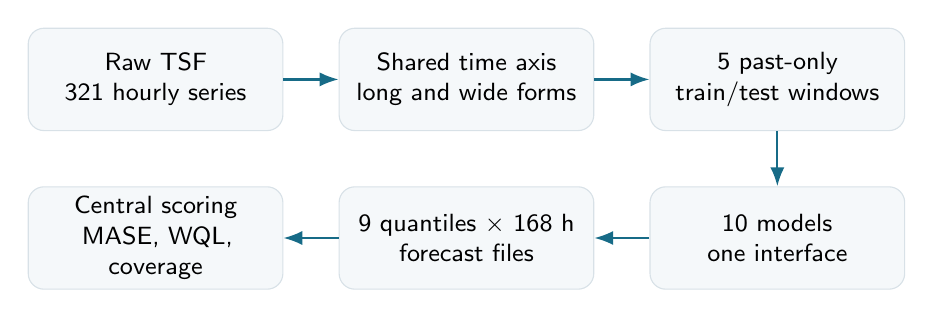
\begin{tikzpicture}[
  node distance=7mm and 7mm,
  box/.style={draw=line,rounded corners=2mm,fill=paper,minimum height=13mm,
              text width=30mm,align=center,font=\small\sffamily},
  arrow/.style={-{Latex[length=2.4mm]},thick,draw=blue}]
  \node[box] (raw) {Raw TSF\\321 hourly series};
  \node[box,right=of raw] (wide) {Shared time axis\\long and wide forms};
  \node[box,right=of wide] (windows) {5 past-only\\train/test windows};
  \node[box,below=of windows] (models) {10 models\\one interface};
  \node[box,left=of models] (forecasts) {9 quantiles $\times$ 168 h\\forecast files};
  \node[box,left=of forecasts] (metrics) {Central scoring\\MASE, WQL, coverage};
  \draw[arrow] (raw) -- (wide);
  \draw[arrow] (wide) -- (windows);
  \draw[arrow] (windows) -- (models);
  \draw[arrow] (models) -- (forecasts);
  \draw[arrow] (forecasts) -- (metrics);
\end{tikzpicture}
\caption{Common evaluation pipeline and leakage controls.}
\label{fig:pipeline}
\end{figure}

Demand forecasts are clipped to be non-negative. A per-series upper bound of ten times the maximum
past value limits numerical explosions. The nine quantiles are sorted at every timestamp to prevent
quantile crossing. These post-processing steps are identical for all models.

% -----------------------------------------------------------------------------
\section{Models Compared}

\subsection{Seasonal-naive and classical models}

Two seasonal-naive methods repeat the last day ($m=24$) or last week ($m=168$). The weekly variant
is the main operational baseline. Because these point forecasts are copied into all nine quantile
columns, their prediction intervals are degenerate and should not be interpreted as genuine
uncertainty estimates.

AutoTheta, AutoETS, and MSTL are fit independently to each series using the most recent 2,016 hours.
MSTL decomposes daily and weekly seasonal components and uses ETS as the trend forecaster. Gaussian
prediction intervals are mapped to the nine evaluation quantiles.

\subsection{Global LightGBM}

LightGBM \cite{ke2017} is trained globally across all series. The target is transformed with a
local per-series standard scaler. Features include lags of 1, 24, 48, 168, and 336 hours; daily and
weekly rolling statistics; hour; day of week; month; and a weekend indicator. Separate models are
fit for $q_{0.1}$, $q_{0.5}$, and $q_{0.9}$, with intermediate quantiles obtained by linear
interpolation.

\subsection{PatchTST trained from scratch}

PatchTST segments the time axis into overlapping patches and shares Transformer weights across
channels \cite{nie2023}. The implementation uses 512 hours of context, patch length 16, stride 8,
three encoder layers, hidden size 128, eight attention heads, and RevIN normalization. Nine
quantiles are learned jointly with a multi-quantile pinball loss.

\subsection{Chronos-Bolt zero-shot and fine-tuned}

Chronos is a family of probabilistic foundation models pretrained on broad collections of time
series \cite{ansari2024}. The saved \code{chronos-bolt-base} configuration accepts up to 2,048
historical steps, divides them into non-overlapping patches of length 16, applies instance
normalization, and passes the result through a T5-based encoder-decoder. The configuration contains
12 encoder and 12 decoder layers, model width 768, 12 attention heads, feed-forward width 3,072,
and dropout 0.1. Its output head directly predicts nine quantiles for the next 64 steps.

The 168-hour horizon is generated in 64-hour blocks. Where the library does not natively allow a
longer prediction length, each block's median forecast is appended to the context before producing
the next block. This median-feedback mechanism is an important potential source of accumulated
error at the end of the horizon.

\begin{table}[htbp]
\centering
\caption{Main configurations of the learned models.}
\label{tab:architectures}
\small
\begin{tabularx}{\textwidth}{@{}lYYY@{}}
\toprule
Property & LightGBM & PatchTST & Chronos-Bolt Base\\
\midrule
Context & 8,760 hours & 512 hours & 2,048 hours\\
Forecast output & 3 quantiles + interpolation & 168 h, 9 quantiles & 64 h, 9 quantiles\\
Normalization & Local standardization & RevIN & Instance normalization\\
Core capacity & 300 trees, 64 leaves & 3 layers, $d=128$ & 12+12 layers, $d=768$\\
Loss & Quantile objective & Multi-quantile loss & Scaled multi-quantile loss\\
Calendar features & Yes & No & No\\
Pretraining & No & No & Yes\\
\bottomrule
\end{tabularx}
\end{table}

% -----------------------------------------------------------------------------
\section{Training and Fine-tuning}

\subsection{PatchTST training}

PatchTST is refit from scratch for every backtest window. The last 168 past hours form a validation
tail. Training uses a learning rate of $10^{-3}$, batch size 32 series, and 256 sampled windows per
step. Validation is checked every 100 steps; training stops after five consecutive checks without
improvement. The 50,000-step limit is only a safety ceiling and is never approached.

\subsection{Chronos-Bolt fine-tuning}

For each backtest window, the model is reinitialized from \code{amazon/chronos-bolt-base}. A
training example consists of a randomly chosen series and time endpoint, a 2,048-hour context, and
the following 64-hour target. The final 64 past hours are excluded from sampling and held out for
validation. All model weights are updated with AdamW at learning rate $10^{-5}$ and batch size 24;
the gradient norm is clipped at 1.0.

Validation is evaluated every 50 steps. If loss fails to improve by more than $10^{-5}$ for five
consecutive checks, training stops and the best checkpoint is restored. Each backtest window is
fine-tuned independently from the pretrained weights. The shareable final model is then trained on
the full history with the same recipe.

\begin{table}[htbp]
\centering
\caption{Observed early-stopping steps.}
\label{tab:stopsteps}
\begin{tabular}{@{}lrrrrrr@{}}
\toprule
Model & W1 & W2 & W3 & W4 & W5 & Full data\\
\midrule
PatchTST & 1,800 & 2,500 & 1,600 & 2,300 & 2,000 & --\\
Chronos-Bolt fine-tuning & 500 & 350 & 650 & 500 & 500 & 400\\
\bottomrule
\end{tabular}
\end{table}

For the full-data fine-tune, the minimum validation loss occurs at step 150. The loop terminates at
step 400 after exhausting patience, then restores the weights from step 150. Therefore, ``400
steps'' describes the duration of the early-stopping loop, not the final checkpoint's weight state.

\begin{figure}[htbp]
\centering
\begin{tikzpicture}
\begin{axis}[
  width=.83\textwidth,height=6.2cm,
  xlabel={Fine-tuning step},ylabel={Validation loss},
  xmin=40,xmax=410,grid=major,grid style={line!55},
  axis line style={line},tick label style={font=\small},label style={font=\small\sffamily},
  scaled y ticks=false]
  \addplot[very thick,teal,mark=*,mark size=1.8pt]
    table[x=step,y=val_loss,col sep=comma]{outputs/train_logs/ft_final_val_curve.csv};
  \addplot[only marks,mark=star,mark size=3.2pt,gold!80!black]
    coordinates {(150,26.8614500364)};
  \node[anchor=south west,font=\small\sffamily,fill=white,inner sep=2pt]
    at (axis cs:155,26.88) {best checkpoint};
\end{axis}
\end{tikzpicture}
\caption{Validation curve for the full-data Chronos-Bolt fine-tune.}
\label{fig:ftcurve}
\end{figure}

% -----------------------------------------------------------------------------
\section{Evaluation Metrics}

Let $y_{t,i}$ denote the observed value, $\hat y_{t,i}$ the median forecast, $T_i$ the training
sample for series $i$, and $m=24$ the seasonal period. Metrics are computed first for each
series-window pair and then averaged equally over 321 series and five windows. This prevents
high-consumption series from dominating the result.

\subsection{Point metrics}

\begin{align}
\operatorname{MAE}_i &= \frac{1}{H}\sum_{t=1}^{H}|y_{t,i}-\hat y_{t,i}|,\\
\operatorname{RMSE}_i &= \sqrt{\frac{1}{H}\sum_{t=1}^{H}(y_{t,i}-\hat y_{t,i})^2},\\
\operatorname{sMAPE}_i &= \frac{100}{H}\sum_{t=1}^{H}
\frac{2|y_{t,i}-\hat y_{t,i}|}{|y_{t,i}|+|\hat y_{t,i}|},\\
\operatorname{MASE}_i &=
\frac{\operatorname{MAE}_i}
{\frac{1}{|T_i|-m}\sum_{t=m+1}^{|T_i|}|y_{t,i}-y_{t-m,i}|}.
\end{align}

MASE is scale-free and supports comparisons across series with different magnitudes
\cite{hyndman2006}. Seasonal-constant series with a zero denominator are excluded from MASE and
counted explicitly. No series-window pair is excluded in this run.

\subsection{Probabilistic metrics}

For quantile $q\in\{0.1,\ldots,0.9\}$, pinball loss is

\begin{equation}
L_q(y,\hat y_q)=\max\{q(y-\hat y_q),(q-1)(y-\hat y_q)\}.
\end{equation}

The project computes Weighted Quantile Loss as

\begin{equation}
\operatorname{WQL}_i =
\frac{2}{9\sum_t |y_{t,i}|}
\sum_{q}\sum_{t=1}^{H} L_q(y_{t,i},\hat y_{q,t,i}).
\end{equation}

Lower WQL is better. Central \SI{80}{\percent} interval coverage is the fraction of observations
for which $q_{0.1}\leq y\leq q_{0.9}$. The nominal target is 0.80. High coverage alone is not
sufficient: unnecessarily wide intervals can cover well while scoring poorly on WQL.

% -----------------------------------------------------------------------------
\section{Experimental Results}

\subsection{Overall ranking}

\Cref{tab:leaderboard} reports all ten models under the common protocol. Models are ranked by the
primary metric, MASE.

\begin{table}[htbp]
\centering
\caption{Overall leaderboard. Down arrows indicate that lower values are better.}
\label{tab:leaderboard}
\scriptsize
\begin{tabular}{@{}lrrrrrrr@{}}
\toprule
Model & MASE$\downarrow$ & sMAPE$\downarrow$ & RMSE$\downarrow$ & MAE$\downarrow$ & WQL$\downarrow$ & Coverage & vs. baseline\\
\midrule
\code{chronos_bolt_base_ft} & \best{0.9358} & 10.83 & \best{223.46} & 150.15 & \best{0.0896} & 0.701 & \best{$-$15.9\%}\\
\code{chronos_bolt_base} & 0.9378 & \best{10.68} & 224.03 & \best{149.06} & 0.0900 & 0.712 & $-$15.7\%\\
\code{chronos_bolt_small} & 0.9754 & 11.11 & 237.02 & 159.25 & 0.0920 & 0.710 & $-$12.4\%\\
\code{seasonal_naive_168} & 1.1130 & 11.71 & 276.12 & 174.21 & 0.1279 & 0.095 & baseline\\
\code{lgbm_global} & 1.2073 & 14.40 & 280.71 & 191.16 & 0.2828 & 0.974 & $+$8.5\%\\
\code{mstl} & 1.2984 & 17.01 & 299.27 & 229.53 & 0.1398 & 0.884 & $+$16.7\%\\
\code{seasonal_naive_24} & 1.2993 & 14.33 & 315.09 & 207.06 & 0.1527 & 0.045 & $+$16.7\%\\
\code{auto_ets} & 1.3988 & 17.40 & 310.21 & 223.10 & 0.2335 & 0.808 & $+$25.7\%\\
\code{patchtst} & 1.7116 & 20.10 & 378.90 & 300.10 & 0.1517 & 0.721 & $+$53.8\%\\
\code{auto_theta} & 1.7528 & 19.93 & 464.24 & 362.77 & 0.2337 & 0.956 & $+$57.5\%\\
\bottomrule
\end{tabular}
\end{table}

\begin{figure}[htbp]
\centering
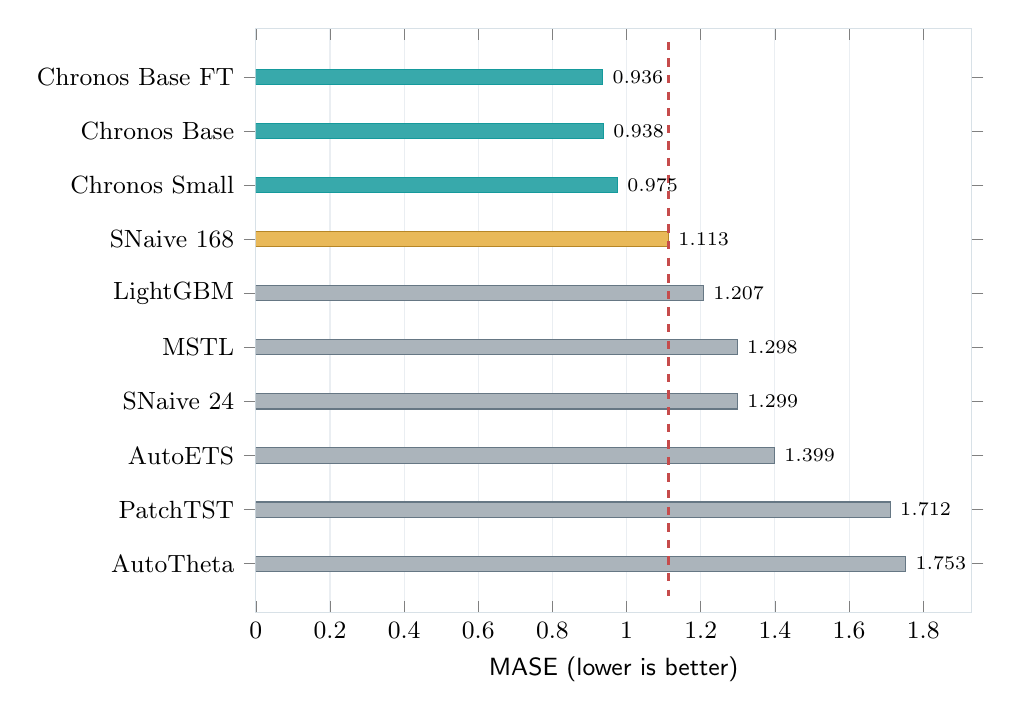
\begin{tikzpicture}
\begin{axis}[
  xbar,bar width=5.5pt,bar shift=0pt,
  width=.88\textwidth,height=9cm,
  xmin=0,xmax=1.93,
  xlabel={MASE (lower is better)},
  ytick={0,1,2,3,4,5,6,7,8,9},
  yticklabels={Chronos Base FT,Chronos Base,Chronos Small,SNaive 168,LightGBM,MSTL,SNaive 24,AutoETS,PatchTST,AutoTheta},
  y dir=reverse,
  tick label style={font=\small},label style={font=\small\sffamily},
  xmajorgrids=true,grid style={line!55},axis line style={line},
  nodes near coords,nodes near coords align={horizontal},
  every node near coord/.append style={font=\scriptsize\sffamily,anchor=west},
  /pgf/number format/fixed,/pgf/number format/precision=3]
  \addplot[fill=teal!85,draw=teal] coordinates {(0.9358,0) (0.9378,1) (0.9754,2)};
  \addplot[fill=gold!80,draw=gold!80!black] coordinates {(1.1130,3)};
  \addplot[fill=muted!55,draw=muted] coordinates {(1.2073,4) (1.2984,5) (1.2993,6)
    (1.3988,7) (1.7116,8) (1.7528,9)};
  \draw[red,dashed,thick] (axis cs:1.113,-.65) -- (axis cs:1.113,9.6);
\end{axis}
\end{tikzpicture}
\caption{Overall MASE. The dashed line is the weekly seasonal-naive baseline.}
\label{fig:maseoverall}
\end{figure}

Three findings stand out:

\begin{itemize}
  \item Only the Chronos-Bolt family beats the weekly seasonal-naive baseline on MASE.
  \item Fine-tuned and zero-shot Chronos-Bolt Base improve MASE by \SI{15.9}{\percent} and
  \SI{15.7}{\percent}, respectively, relative to that baseline.
  \item The WQL gap is larger: 0.0896 for fine-tuned Chronos is \SI{35.9}{\percent} lower than
  MSTL's 0.1398, the best WQL among the reasonably calibrated classical alternatives.
\end{itemize}

Fine-tuned Chronos ranks first on MASE, RMSE, and WQL, but zero-shot Chronos Base is slightly better
on sMAPE and MAE. The results therefore do not support a claim of superiority on every metric.

\subsection{Window-level results and the Christmas effect}

\begin{figure}[htbp]
\centering
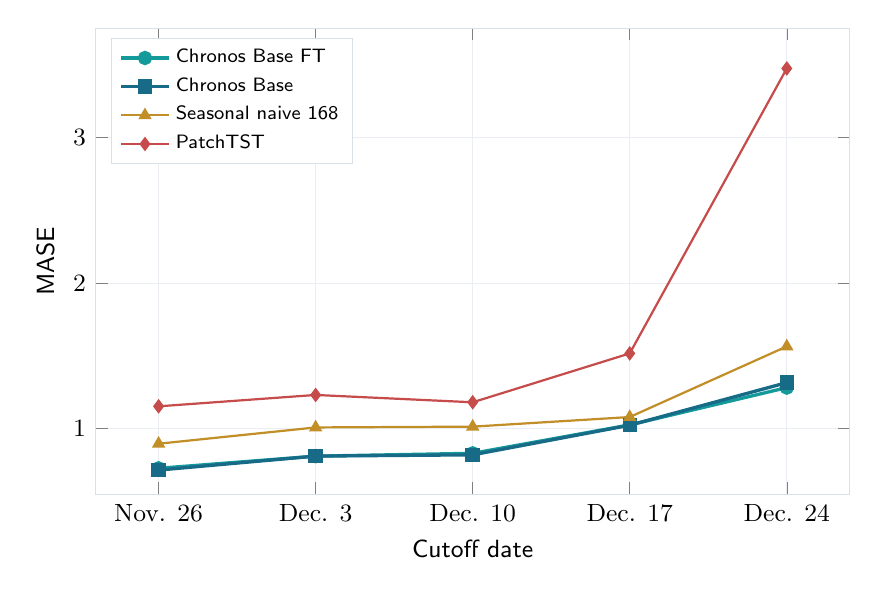
\begin{tikzpicture}
\begin{axis}[
  width=.92\textwidth,height=7.5cm,
  xlabel={Cutoff date},ylabel={MASE},
  xtick={0,1,2,3,4},
  xticklabels={Nov. 26,Dec. 3,Dec. 10,Dec. 17,Dec. 24},
  ymin=.55,ymax=3.75,
  grid=major,grid style={line!55},axis line style={line},
  tick label style={font=\small},label style={font=\small\sffamily},
  legend style={at={(0.02,0.98)},anchor=north west,draw=line,fill=white,font=\scriptsize\sffamily},
  legend cell align=left]
  \addplot[very thick,teal,mark=*] coordinates {(0,.7282)(1,.8115)(2,.8310)(3,1.0261)(4,1.2821)};
  \addlegendentry{Chronos Base FT}
  \addplot[very thick,blue,mark=square*] coordinates {(0,.7159)(1,.8120)(2,.8206)(3,1.0240)(4,1.3165)};
  \addlegendentry{Chronos Base}
  \addplot[thick,gold!85!black,mark=triangle*] coordinates {(0,.8969)(1,1.0087)(2,1.0141)(3,1.0802)(4,1.5651)};
  \addlegendentry{Seasonal naive 168}
  \addplot[thick,red,mark=diamond*] coordinates {(0,1.1536)(1,1.2318)(2,1.1814)(3,1.5170)(4,3.4739)};
  \addlegendentry{PatchTST}
\end{axis}
\end{tikzpicture}
\caption{MASE across the five backtest windows. The final cutoff forecasts December 25--31.}
\label{fig:windowmase}
\end{figure}

\begin{table}[htbp]
\centering
\caption{Window-level MASE for selected models.}
\label{tab:windowmase}
\begin{tabular}{@{}lrrrrr@{}}
\toprule
Model & Nov. 26 & Dec. 3 & Dec. 10 & Dec. 17 & Dec. 24\\
\midrule
Chronos Base FT & 0.728 & 0.812 & 0.831 & 1.026 & \best{1.282}\\
Chronos Base & \best{0.716} & \best{0.812} & \best{0.821} & \best{1.024} & 1.317\\
Seasonal naive 168 & 0.897 & 1.009 & 1.014 & 1.080 & 1.565\\
LightGBM & 0.910 & 1.051 & 1.120 & 1.197 & 1.759\\
PatchTST & 1.154 & 1.232 & 1.181 & 1.517 & 3.474\\
\bottomrule
\end{tabular}
\end{table}

Every model deteriorates in the December 25--31 window. PatchTST's MASE rises to 3.474, while
Chronos remains between 1.28 and 1.32. PatchTST sees only past target values and has no explicit
calendar input, making the holiday regime change difficult to anticipate. Chronos also has no
calendar covariate, so the gap cannot be attributed solely to calendar awareness. More general
patterns learned in pretraining and earlier holiday episodes in the fine-tuning data are plausible
explanations.

\subsection{What fine-tuning contributes}

The overall difference between fine-tuned and zero-shot Chronos-Bolt Base is only 0.0020 MASE,
about \SI{0.22}{\percent}, and 0.0004 WQL. Across the first four windows, the fine-tuned minus
zero-shot MASE differences are $+0.0123$, $-0.0005$, $+0.0104$, and $+0.0021$. Fine-tuning is
therefore roughly level or slightly worse on ordinary weeks. In the final window, however, the
difference is $-0.0344$, a relative MASE improvement of about \SI{2.6}{\percent}.

At the series level in the Christmas window, fine-tuning produces lower MASE for 187 of 321 series
(\SI{58.3}{\percent}). Under equal win probability, the exact one-sided sign-test result is
$p=0.0018$. The WQL win count is 183/321. Across all windows and series, however, fine-tuning beats
zero-shot Base only about \SI{44}{\percent} of the time.

\begin{caution}[Appropriate interpretation]
  The evidence does not support the claim that fine-tuning is better everywhere. A narrower claim
  is supported: \emph{fine-tuning preserved average performance and was more robust in the single
  clearly anomalous test week}. This robustness observation should be validated on other years and
  exceptional periods.
\end{caution}

\subsection{Breadth of gains and scale sensitivity}

Fine-tuned Chronos beats the weekly seasonal naive on 1,255 of 1,605 series-window pairs
(\SI{78.2}{\percent}); zero-shot Base does so on 1,273 pairs (\SI{79.3}{\percent}). Fine-tuned
Chronos beats PatchTST on 1,524 pairs (\SI{95.0}{\percent}). The average gain is therefore not
driven by only a few high-volume series.

When series are grouped into terciles by mean consumption, fine-tuned Chronos achieves MASE values
of 0.924, 0.949, and 0.934 for small-, medium-, and large-scale series. The corresponding weekly
seasonal-naive values are 1.107, 1.138, and 1.094. Per-series normalization appears to support
balanced performance across scales.

\subsection{Probabilistic calibration}

\begin{table}[htbp]
\centering
\caption{Empirical coverage of nominal \SI{80}{\percent} intervals.}
\label{tab:coverage}
\begin{tabularx}{.86\textwidth}{@{}l r Y@{}}
\toprule
Model group & Coverage & Interpretation\\
\midrule
Chronos-Bolt family & 0.70--0.71 & Intervals are roughly 9--10 percentage points too narrow\\
PatchTST & 0.721 & Too narrow; coverage falls to 0.543 in the Christmas window\\
AutoETS & 0.808 & Near nominal, but point accuracy is weak\\
MSTL & 0.884 & Somewhat wide\\
LightGBM / AutoTheta & 0.974 / 0.956 & Far too wide; high coverage alone is not success\\
Seasonal naives & 0.045--0.095 & Degenerate because they are point forecasts\\
\bottomrule
\end{tabularx}
\end{table}

Chronos combines low WQL with undercoverage. Fine-tuning reduces coverage from 0.712 to 0.701. If
production use requires reliable coverage, the $q_{0.1}$--$q_{0.9}$ interval should be widened with
a series- or group-level conformal correction learned only from past calibration residuals.

% -----------------------------------------------------------------------------
\section{Compute Environment and Reproducibility}

The benchmark was run on an NVIDIA A100-SXM4-40GB with random seed 42. Recorded software versions
are listed in \cref{tab:environment}.

\begin{table}[htbp]
\centering
\caption{Recorded run environment.}
\label{tab:environment}
\begin{tabular}{@{}ll@{}}
\toprule
Component & Version / value\\
\midrule
GPU & NVIDIA A100-SXM4-40GB\\
PyTorch & 2.11.0+cu128\\
NumPy / pandas & 2.0.2 / 2.2.2\\
StatsForecast / MLForecast & 2.0.3 / 1.0.31\\
LightGBM & 4.6.0\\
NeuralForecast & 3.1.9\\
chronos-forecasting & 1.5.3\\
\bottomrule
\end{tabular}
\end{table}

The benchmark notebook performs data loading, window construction, training or inference for all
ten models, centralized scoring, training-log export, and final model serialization. Documented
end-to-end runtime on an A100 is about 1.5--2.5 hours. The final model is saved in Hugging Face
format as \code{config.json} and \code{model.safetensors}; a reload-and-predict test verifies a
168-hour output for all 321 series.

To reproduce the run:

\begin{enumerate}
  \item Open \sourcepath{energy_forecasting_foundation_models.ipynb} in a GPU environment.
  \item Review the data path and frozen protocol before running models. Do not revise the protocol
  after inspecting results.
  \item Run all cells in order. Archive \sourcepath{outputs/run_meta.json} and the
  leaderboard in \sourcepath{outputs/metrics/}.
  \item Reload the saved model and evaluate coverage and distribution shift on independent data
  before production use.
\end{enumerate}

Published model:
\href{https://huggingface.co/mskayacioglu/chronos-bolt-base-monash-electricity-hourly}
{mskayacioglu/chronos-bolt-base-monash-electricity-hourly}.

% -----------------------------------------------------------------------------
\section{Limitations and Validity Threats}

\begin{itemize}
  \item \textbf{One dataset and one frequency:} Results are specific to 321 hourly electricity
  series and do not automatically generalize to other countries, climates, frequencies, or demand
  definitions.
  \item \textbf{Five test weeks:} The test period contains only the final five weeks of 2014. Other
  seasons, heat waves, price shocks, and holidays are not represented.
  \item \textbf{One anomalous episode:} The fine-tuning robustness gain is observed in one Christmas
  week and is not a multi-event study.
  \item \textbf{No exogenous variables:} Weather, holidays, prices, and customer information are not
  supplied to Chronos or PatchTST, despite their likely importance during exceptional periods.
  \item \textbf{Model-selection budget:} The protocol is frozen, but each model family does not
  receive an equally extensive hyperparameter search. Results compare reasonable recipes rather
  than each family's theoretical optimum.
  \item \textbf{Interval calibration:} Chronos does not attain nominal \SI{80}{\percent} coverage;
  uncalibrated use can understate uncertainty.
  \item \textbf{Long-horizon rolling:} Chronos extends its native 64-step output with median
  feedback, which can accumulate error in later blocks.
\end{itemize}

% -----------------------------------------------------------------------------
\section{Conclusion and Recommended Use}

The recommended model for this benchmark is \code{chronos_bolt_base_ft}. It ranks first on the
primary MASE metric and WQL, performs consistently across scale groups, and is more robust than the
zero-shot model in the hardest test week. However, \code{chronos_bolt_base} is only 0.002 MASE
behind and requires no dataset-specific training, making it a strong lower-cost operational option.
Where foundation-model deployment is unavailable, the weekly seasonal naive remains a reliable and
surprisingly competitive fallback.

\begin{finding}[Decision summary]
\begin{tabularx}{\textwidth}{@{}lY@{}}
\textbf{Highest benchmark accuracy} & Fine-tuned Chronos-Bolt Base\\
\textbf{Strong training-free option} & Zero-shot Chronos-Bolt Base\\
\textbf{Lowest-complexity fallback} & Weekly seasonal naive\\
\textbf{Required pre-production step} & Backtest on new periods and calibrate quantiles\\
\textbf{Priority extension} & Add weather and holiday covariates; test multiple anomalous periods\\
\end{tabularx}
\end{finding}

% -----------------------------------------------------------------------------
\appendix
\section{Detailed Hyperparameters}

\begin{longtable}{@{}p{35mm}p{43mm}p{74mm}@{}}
\caption{Main implementation hyperparameters.}\label{tab:hyperparams}\\
\toprule
Model / component & Parameter & Value\\
\midrule
\endfirsthead
\toprule
Model / component & Parameter & Value\\
\midrule
\endhead
General & Horizon / windows & 168 hours / 5 windows\\
General & Quantiles & 0.1, 0.2, $\ldots$, 0.9\\
General & Clipping & $[0,10\times\text{past maximum}]$\\
Classical & Context & 2,016 hours\\
MSTL & Seasonalities & 24 and 168; ETS trend forecaster\\
LightGBM & Context & 8,760 hours\\
LightGBM & Lags & 1, 24, 48, 168, 336\\
LightGBM & Trees / leaves & 300 / 64\\
LightGBM & Learning rate & 0.05\\
LightGBM & Minimum child samples & 200\\
LightGBM & Row / column sampling & 0.8 / 0.9\\
PatchTST & Input / horizon & 512 / 168\\
PatchTST & Patch / stride & 16 / 8\\
PatchTST & Hidden / heads / layers & 128 / 8 / 3\\
PatchTST & Dropout & 0.2\\
PatchTST & Learning rate & $10^{-3}$\\
PatchTST & Batch / window batch & 32 / 256\\
PatchTST & Validation / patience & Every 100 steps / 5 checks\\
Chronos-Bolt & Context / native horizon & 2,048 / 64\\
Chronos-Bolt & Patch / stride & 16 / 16\\
Chronos-Bolt & Model width / heads & 768 / 12\\
Chronos-Bolt & Encoder / decoder & 12 / 12 layers\\
Chronos-Bolt & Feed-forward / dropout & 3,072 / 0.1\\
Fine-tuning & Optimizer & AdamW, learning rate $10^{-5}$\\
Fine-tuning & Batch / target & 24 / 64 hours\\
Fine-tuning & Gradient clipping & 1.0\\
Fine-tuning & Validation / patience & Every 50 steps / 5 checks\\
\bottomrule
\end{longtable}

\section{Artifact Traceability}

\begin{tabularx}{\textwidth}{@{}lY@{}}
\toprule
File & Use in this report\\
\midrule
\sourcepath{energy_forecasting_foundation_models.ipynb} & Data loading, model definitions, training, and evaluation\\
\sourcepath{outputs/metrics/leaderboard.csv} & Overall ranking and headline metrics\\
\sourcepath{outputs/metrics/*_by_window.csv} & Window-level MASE, WQL, and coverage\\
\sourcepath{outputs/metrics/*_per_series.csv} & Paired win rates and sign-test counts\\
\sourcepath{outputs/train_logs/} & Early-stopping steps and validation curves\\
\sourcepath{outputs/run_meta.json} & Hardware, software versions, and observed stop steps\\
\sourcepath{outputs/models/chronos_bolt_base_ft/config.json} & Saved Chronos-Bolt architecture\\
\bottomrule
\end{tabularx}

% -----------------------------------------------------------------------------
\clearpage
\begin{thebibliography}{9}

\bibitem{ansari2024}
A. F. Ansari, L. Stella, C. Turkmen, et al.,
``Chronos: Learning the Language of Time Series,''
\emph{Transactions on Machine Learning Research}, 2024.
\url{https://openreview.net/forum?id=gerNCVqqtR}

\bibitem{godahewa2021}
R. Godahewa, C. Bergmeir, G. I. Webb, R. J. Hyndman, and P. Montero-Manso,
``Monash Time Series Forecasting Archive,''
\emph{NeurIPS Datasets and Benchmarks}, 2021.
\url{https://arxiv.org/abs/2105.06643}

\bibitem{nie2023}
Y. Nie, N. H. Nguyen, P. Sinthong, and J. Kalagnanam,
``A Time Series is Worth 64 Words: Long-term Forecasting with Transformers,''
\emph{International Conference on Learning Representations}, 2023.
\url{https://arxiv.org/abs/2211.14730}

\bibitem{ke2017}
G. Ke, Q. Meng, T. Finley, et al.,
``LightGBM: A Highly Efficient Gradient Boosting Decision Tree,''
\emph{Advances in Neural Information Processing Systems}, vol. 30, 2017.
\url{https://proceedings.neurips.cc/paper_files/paper/2017/hash/6449f44a102fde848669bdd9eb6b76fa-Abstract.html}

\bibitem{hyndman2006}
R. J. Hyndman and A. B. Koehler,
``Another Look at Measures of Forecast Accuracy,''
\emph{International Journal of Forecasting}, vol. 22, no. 4, pp. 679--688, 2006.

\end{thebibliography}

\end{document}
